\documentclass[12pt]{article} % use larger type; default would be 10pt
\usepackage{graphicx,amsmath,subfigure} % support the \includegraphics command and options
\usepackage[pdftex]{color}
\usepackage{natbib}
\usepackage{authblk}


\addtolength{\oddsidemargin}{-.5in}%
\addtolength{\evensidemargin}{-.5in}%
\addtolength{\textwidth}{1in}%
\addtolength{\textheight}{1.3in}%
\addtolength{\topmargin}{-.8in}%

\begin{document}


\def\spacingset#1{\renewcommand{\baselinestretch}%
{#1}\small\normalsize} \spacingset{1}
\newcommand{\ac}[1]{[{\color{red}\ Andy Says: {\tt #1}}]}
\newcommand{\xc}[1]{[{\color{red}\ Xinran Says: {\tt #1}}]}
\newcommand{\lc}[1]{[{\color{red}\ Lucas Says: {\tt #1}}]}
\newcommand{\mc}[1]{[{\color{red}\ Marcos Says: {\tt #1}}]}
\newcommand{\yc}[1]{[{\color{red}\ Yuhyun Says: {\tt #1}}]}



%%%%%%%%%%%%%%%%%%%%%%%%%%%%%%%%%%%%%%%%%%%%%%%%%%%%%%%%%%%%%%%%%%%%%%%%%%%%%%




  \title{\bf What's in your Wallet? \emph{ Lots of receipts.}}
  \author{Marcos Carzolio, Andy Hoegh, Xinran Hu, Lucas Robers, Yuhyun Song\\ Department of Statistics, Virginia Tech}
 \maketitle
\bigskip
\begin{abstract}
\noindent
\ac{Fill this in}
\end{abstract}

\subsection{Judging: \emph{to be removed after writing}}
\begin{enumerate}
\item Performance of the statistical model evaluated on a validation sample.
\item Creativity of the candidate variables and intuition behind selected model features
\item A written proposal, describing how your tool addressed the aforementioned ``VP questions" \ac{Need to tailor document to these questions}
\end {enumerate}
Teams will score up to 20 points in each category for a maximum score of 60 points, top 5 teams are semi-finalists.


\newpage


\section{Overview of Solution} 
Predicting human behavior is notoriously challenging.  However, in this ``big data'' era massive amounts of information available through data sources such as social media and transaction histories make this problem more manageable.  Furthermore, intelligent and responsible use of big data can benefit all involved parties.  In particular within the context of predicting consumer transactions, customers can be provided with coupons for discounts at merchants which also provides additional business for merchants and instills customer loyalty for the credit card company.  This process supports Capital One's mission of \emph{Making Banking Better for Good}.  

Our predictive modeling scheme can be described in a series of four steps: feature extraction, customer segmentation, predictive modeling, and optimal decision.  An overview of each is provided directly below.
\subsection*{Feature Extraction} 
Raw transaction data does not lend itself directly to predictive modeling.  This is a common trait of massive, and often unstructured data which require preprocessing and feature extraction to retain signals and filters noise present in the information.  In addition to past history at a particular merchant, we also look at customer specific information such as transaction count by industry type, transaction frequency, number of zip codes shopped in and customer--merchant specific variables such as whether the customer shops in a zip code where the merchant is present.  A complete list of variables (more than 270) can be seen below.  

\subsection*{Customer Segmentation:} 
In an ideal scenario the target customers would be drawn the same population; hence, allowing a single modeling framework to be applied to the entire set of customers.  This is clearly not the case with the data set presented in this competition.  The transaction records indicated  heterogenous segments of customers.  So a model based clustering approach was used to segment the customers, then a separate model was applied to each segment.  This makes intuitive sense and results in more accurate predictions. 

\subsection*{Model Building:} 
For each segmentation of customers, a collection of well established classification tools were used to evaluate performance.  Given that our feature set contained so many variables we favored methods that encourage some sparsity in the covariate space, with the random forest algorithm ultimately being selected.  For our response, we extract whether each customer shops at a specified merchant during the three month period for which predictions are needed.  It should be noted that these models are computing the probability of shopping at a merchant in a univariate manner.  This has the built in assumption that the probabilities of visiting separate merchants are independent.  To lessen the correlation structure, indicator variables for shopping at other target merchants are introduced.

\subsection*{Model Use:} 
Given the goal of the project is to make a decision on issuing coupons for each customer, statistical decision theory prove useful when determining the optimal decision for each customer.  The question boils down to the expected return for issuing coupons to a customer.  The mathematical details are provided later on, but five coupons are issued if the expected `gain' is greater than the \$1 penalty for not issuing a coupon.\\

The following sections will provided additional details on each of the four components that go into our modeling framework.  Then a discussion section will follow identify some closing thoughts and touching on some ideas for future work in this area. 
\section{Data Preparation}
\subsection{Feature Extraction}
Much effort was taken to extract meaningful features from the transaction level data.  The key is reducing the data while obtaining information relevant to where a customer may shop in the future.  All variables are constructed on the twelve month period, with the exception of small frequency customers.  These customers have variables constructed on only nine months as three are held out of the validation set for model citing.  A list of customer specific variables are shown below.
\small
\begin{itemize}
\item proportion of purchases online 
\item transaction count by industry (for all purchases and online purchases)
\item total transaction count and transaction count for last 3 months
\item number of zip codes for which purchases are made
\item number of merchants customer shopped at
\end{itemize}
\normalsize
These variables are also used in the cluster segmentation scheme.   The customer-- merchant specific variables are as follows:
\small
\begin{itemize}
\item frequency of shopping at merchant
\item merchant located in customer's home zipcode
\item merchant located in zip code customer regularly shops at
\item customer shop at competitor (same industry)
\item customer shop at competitor in same zip code
\end{itemize}
\normalsize

\subsection{Customer Segmentation}
There are two reasons clustering is both useful and necessary in this scenario.  First, as described there is heterogeneity in the customers - suggesting separate models for intuitive and predictive advantages.  The second is the inclusion of low frequency customers in the validation set.  Fitting a model on customers with high credit card use and then applying it to these low use customers would be a classic interpolation error.

To differentiate heterogenous groups, K-means clustering is applied to three constructed variables: total transactions, number of merchants, number of zip codes shopped in.  The goal is to identify homogenous groups of shoppers so that their behavior can be modeled in the same framework.
\begin{figure}[h!]
\centering
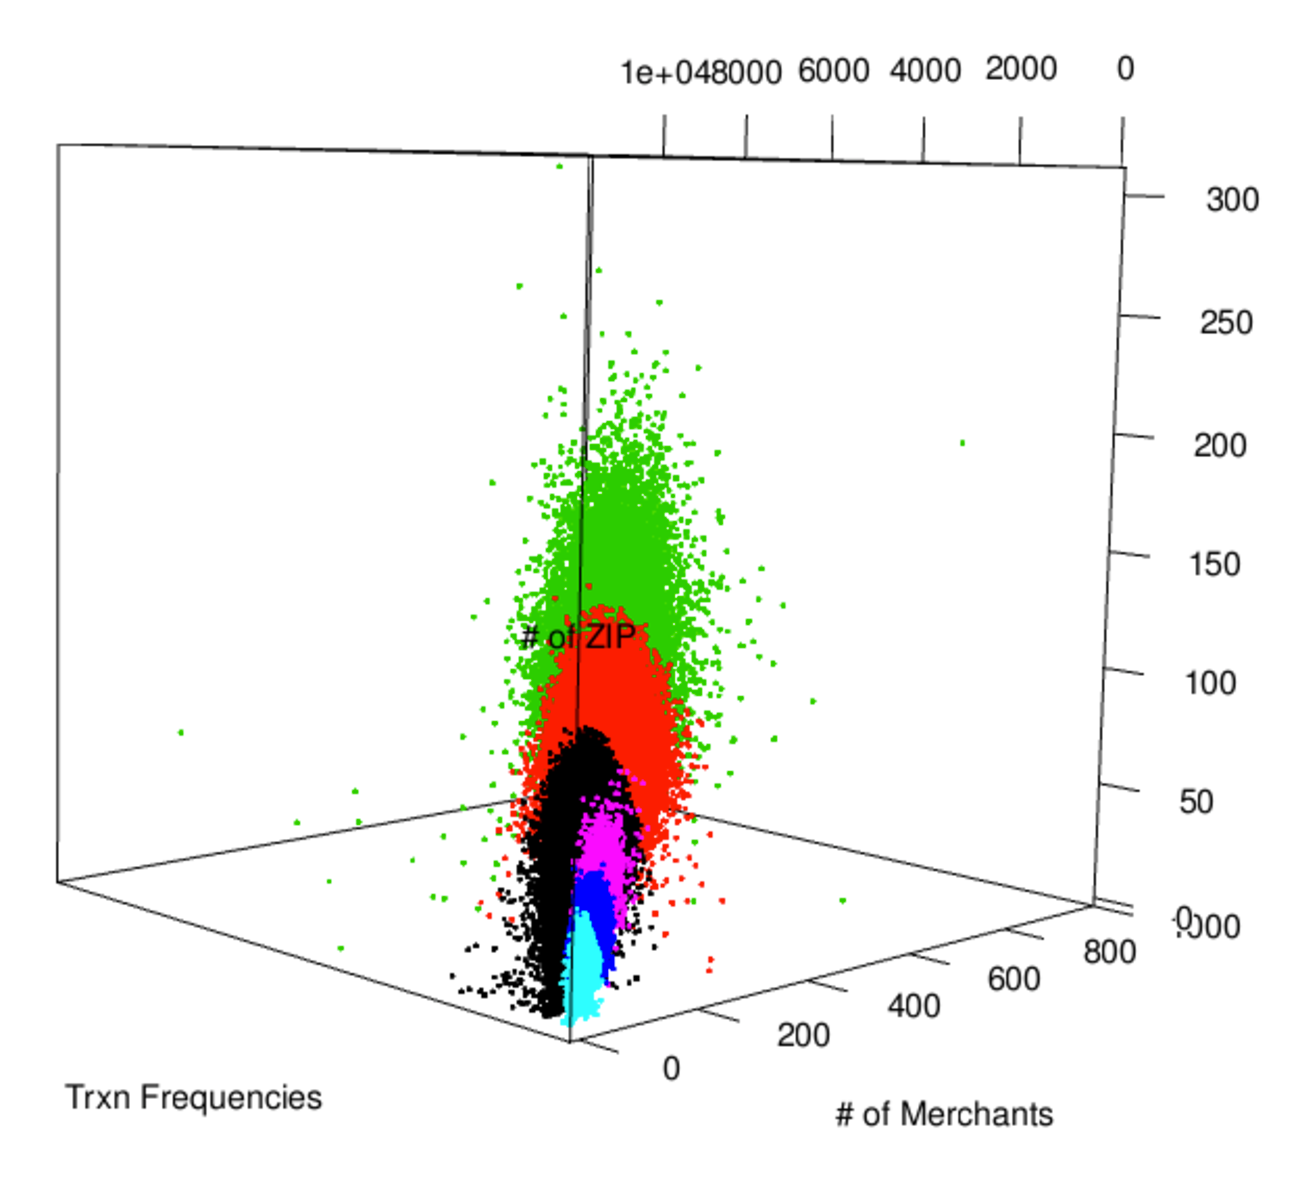
\includegraphics[width=6in]{k_means.pdf}
\label{fig:cluster}
\end{figure}
Figure~\ref{fig:cluster} provides a visual of the constructed clusters.  These clusters break apart customers not only by total transactions, but also take into account the diversity of stores and locales a credit card is used in.

The second reason for clustering is the inclusion of small frequency customers with less than 360 annual transactions in the validation set.  These customers clearly exhibit different spending habits than the high frequency customers that are provided in the sample test sets.  This necessitated a bit of creative thinking to develop a different type of model for these customers.  There were three options: use the models constructed on high frequency customers, do not issue coupons to these customers, or use the 12 months of data to learn about these customers.  Given that options one and two were unsatisfactory, we choose option three.  While not a perfect scenario, it was the best option. 

\section{Model Building}
The random forest algorithm is an ensemble classifier that builds a series of uncorrelated trees which are combined to create a stronger classifier.  Each tree is constructed on a randomly selected subset of data and predictors.  In many problems of this type, the goal is accuracy in the classification itself.  In this case, the importance lies in accurately estimating the class probabilities.  Class probabilities of a random forest algorithm are obtained as the proportion of trees that make a specification classification.

As mentioned earlier, these models assume independence in the probabilities of shopping at merchants.  In reality, there is likely some correlation.  For computational and actual time constraints we estimated the probabilities separately, but included variables denoting whether a customer shopped at another target merchant in our model.  These will adjust the probabilities accordingly.  A more complete solution could be achieved through a multivariate probit model or using a copula.
 
\section{Model Use}
Given the probabilities of a customer shopping at a merchant and and the specified loss function:  
\begin{eqnarray*}
L(\delta,C_i) &=& 3 \text {  offer suite issued with no redemption}\\
&=& -5 * n \text{  offer suite issued with n coupons redeemed}\\
&=& 1 \text{  no offer suite extended},
\end{eqnarray*}
an optimal decision can be made to minimize risk.  That is, for each customer we seek to maximize the expected return:
\begin{eqnarray}
E(return_{issue}) = \$25 P_5 + \$20 P_4 + \$15 P_3 +\$10 P_2 +\$5 P_1 - \$3 P_0,
\end{eqnarray}
where $P_i$ is the probability of $i$ coupons being redeemed.  If $E(return_{issue}) > E(return_{issue}) =-\$1$ then coupons are issued.
\section{Discussion}
While this algorithm is specifically tuned for the merchants specified in the validation test set, the implementation could easily be applied to any merchant.  One subtle, but important aspect about this competition is that the models are designed to predict where a customer will shop in upcoming months -- without any influence from an issued coupon.  As the problem statements outlines, merchants are not as interested in providing discounts to frequent customers, but would like to identify new sets of customers.  Our framework uses features that would help find these customers, in particular a feature has been constructed to identify a merchant's competitor's customers.  The predictive power of this variable is minimal in the current scenario; however, issuing a coupon would cause a behavioral adjustment that may cause a customer to visit a merchant they ordinarily would not.  An interesting evolution that would be particularly interesting for Capital One's business partners would be to conduct an experiment be issuing coupons to customers in order to model behavioral change.    The resultant summary could show the difference in probability of a customer (or more likely a segmentation of customers)  visiting a merchant after being issued a coupon.  In a similar vein our group discussed the concept of a shared merchant that could be analyzed in the same framework as transaction data (e.g. the beer and diapers example).  As a concrete example, perhaps users who shop at Target also often shop at Pier 1.
\end{document}





